\section{Results and Diagnostic Analysis}
\label{sec:evaluation}

\begin{table}[t]
  \caption{Successful tasks out of 100. G and R denote \texttt{gpt-5.6-sol} and \texttt{grok-4.6}. Each workload uses the same targets for all listed configurations.}
  \label{tab:success}
  \begin{tabular*}{\columnwidth}{@{\extracolsep{\fill}}lrrr@{}}
    \toprule
    Agent & ScienceWorld G & DBBench G & DBBench R \\
    \midrule
    No Memory       & 28 & 66 & 65 \\
    Voyager-style   & 42 & 66 & 66 \\
    Reflexion-style & 38 & 64 & 68 \\
    ExpeL-style     & 35 & 65 & 65 \\
    MemGPT-style    & 42 & 64 & 68 \\
    MCMA-style      & 33 & 64 & 66 \\
    AgentKB-style   & 39 & 64 & 66 \\
    \SM{}           & 85 & 67 & 58 \\
    \bottomrule
  \end{tabular*}
\end{table}

\begin{figure*}[t]
  \centering
  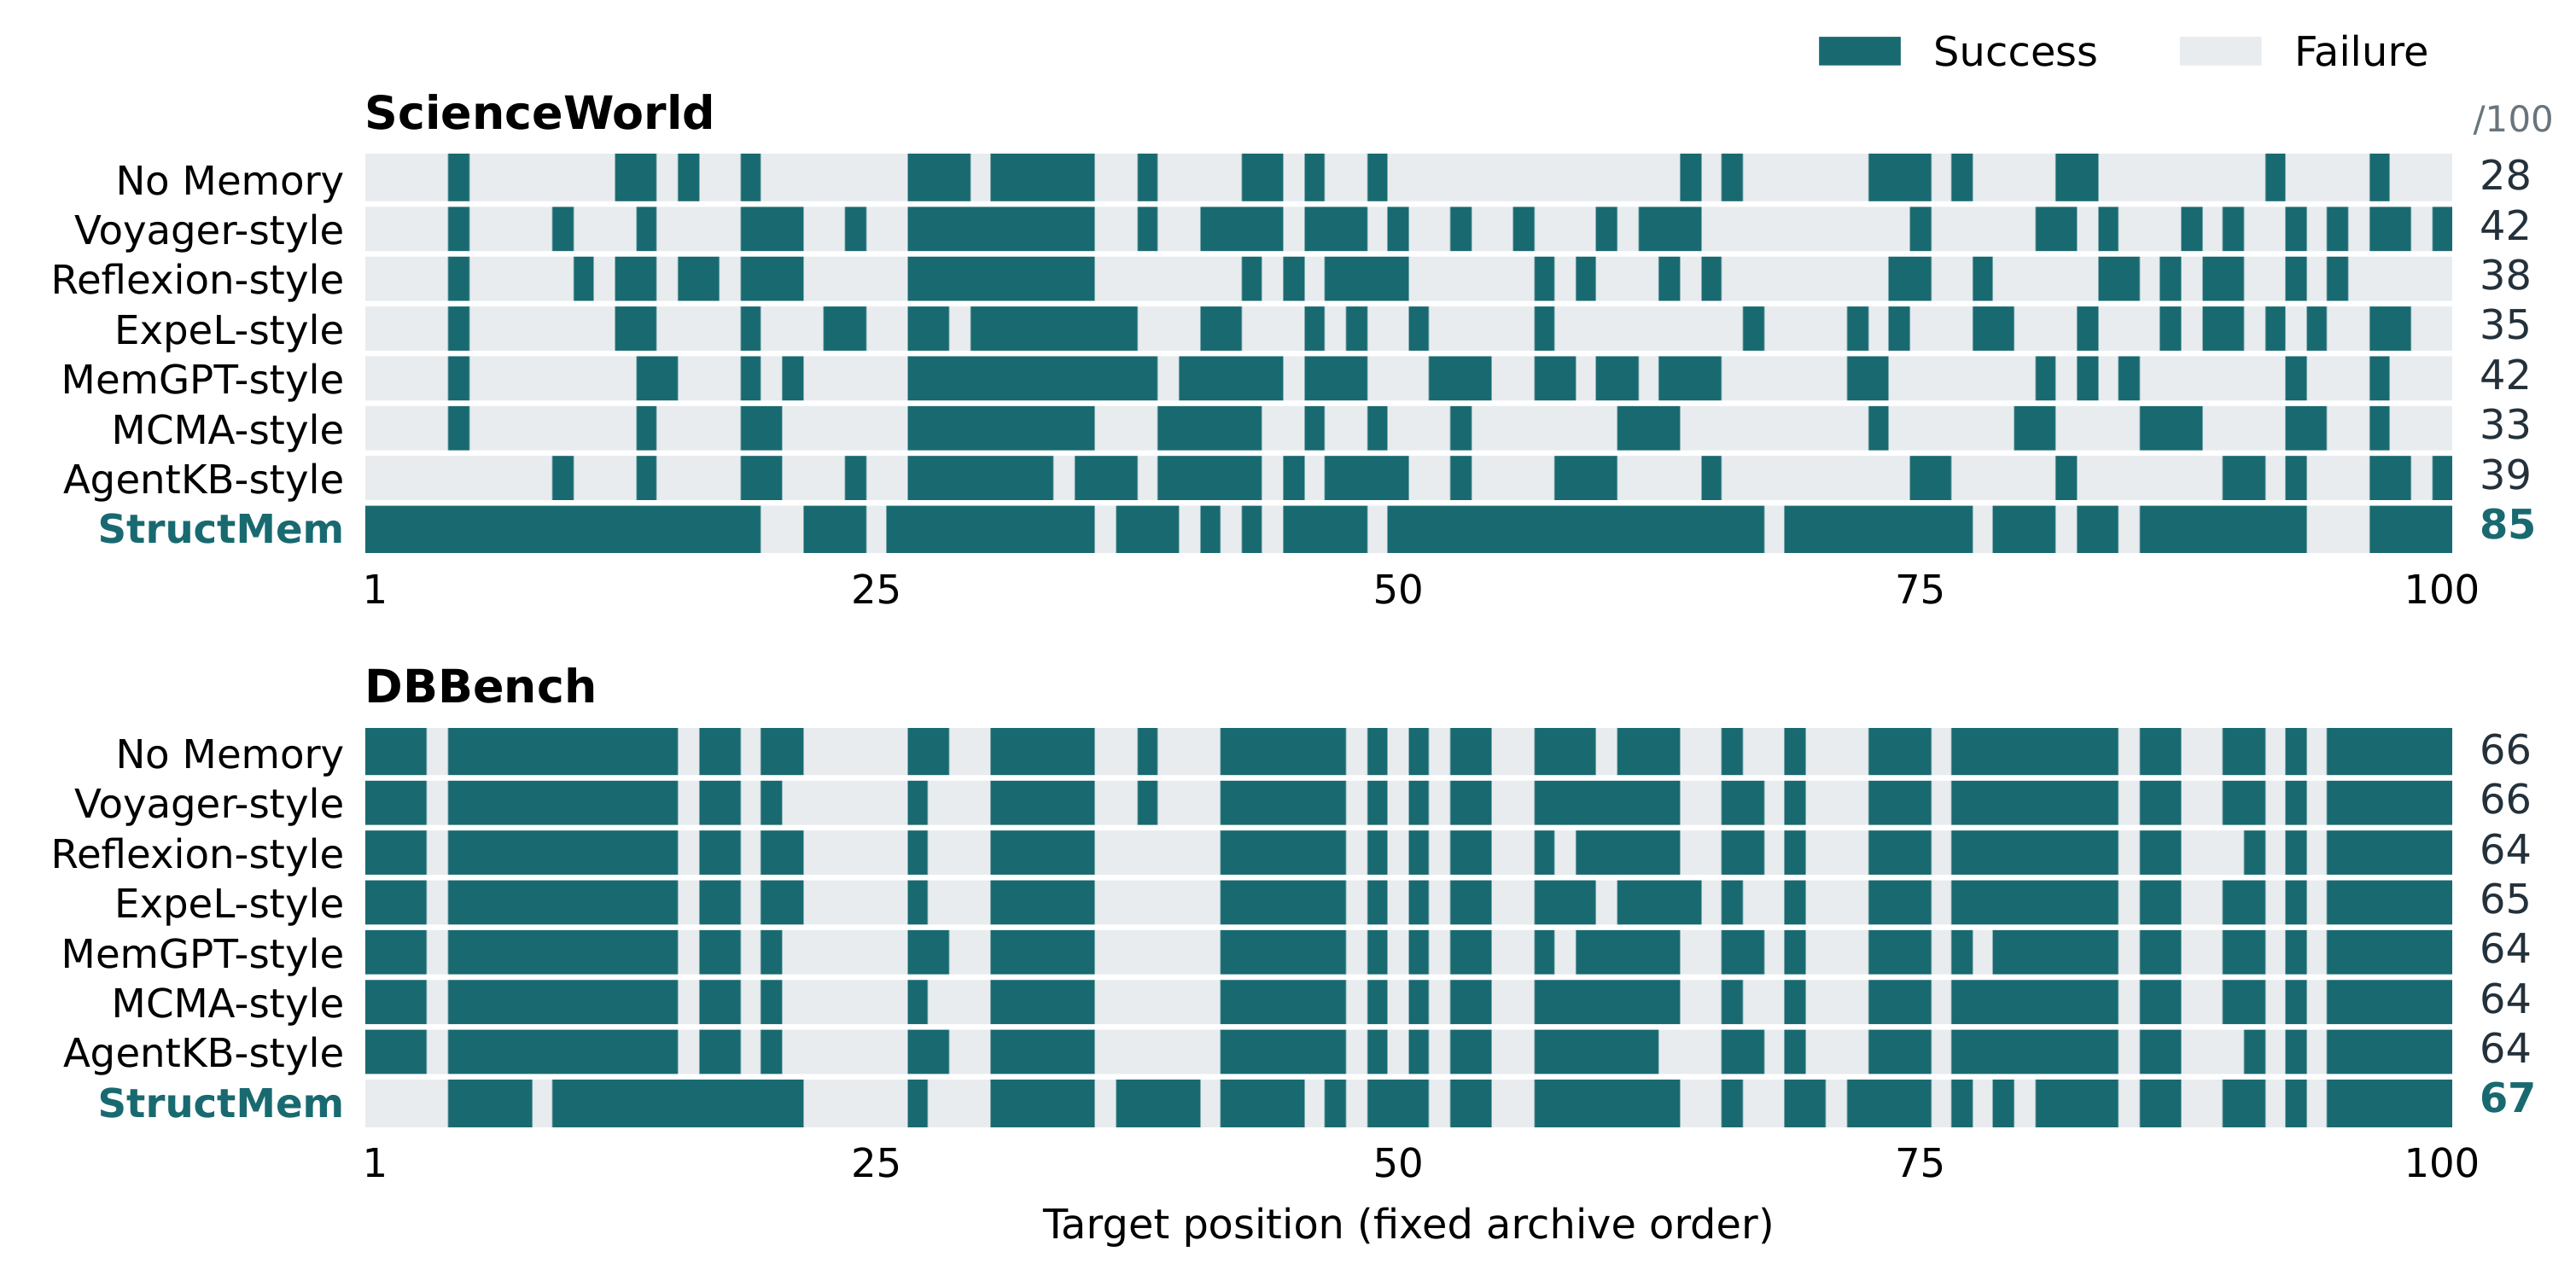
\includegraphics[width=\textwidth]{figures/formal-outcomes.png}
  \caption{Task outcomes on the primary endpoint. Each column represents the same target across rows. Targets follow the fixed archive order and retain both successful and unsuccessful terminal outcomes.}
  \Description{Two outcome matrices show the success or failure of eight agents on each of 100 ScienceWorld and 100 DBBench tasks.}
  \label{fig:task-outcomes}
\end{figure*}

\subsection{Integrated effectiveness}
\label{sec:effectiveness}
Table~\ref{tab:success} shows a large gap on ScienceWorld. The integrated agent succeeds on 85 tasks, compared with 28 for No Memory and 42 for each of Voyager-style and MemGPT-style. On DBBench, it succeeds on one more task than No Memory. The task outcomes in Figure~\ref{fig:task-outcomes} show considerable alignment among DBBench comparators on which queries succeed. ScienceWorld shows more variation across agents.

\begin{figure}[t]
  \centering
  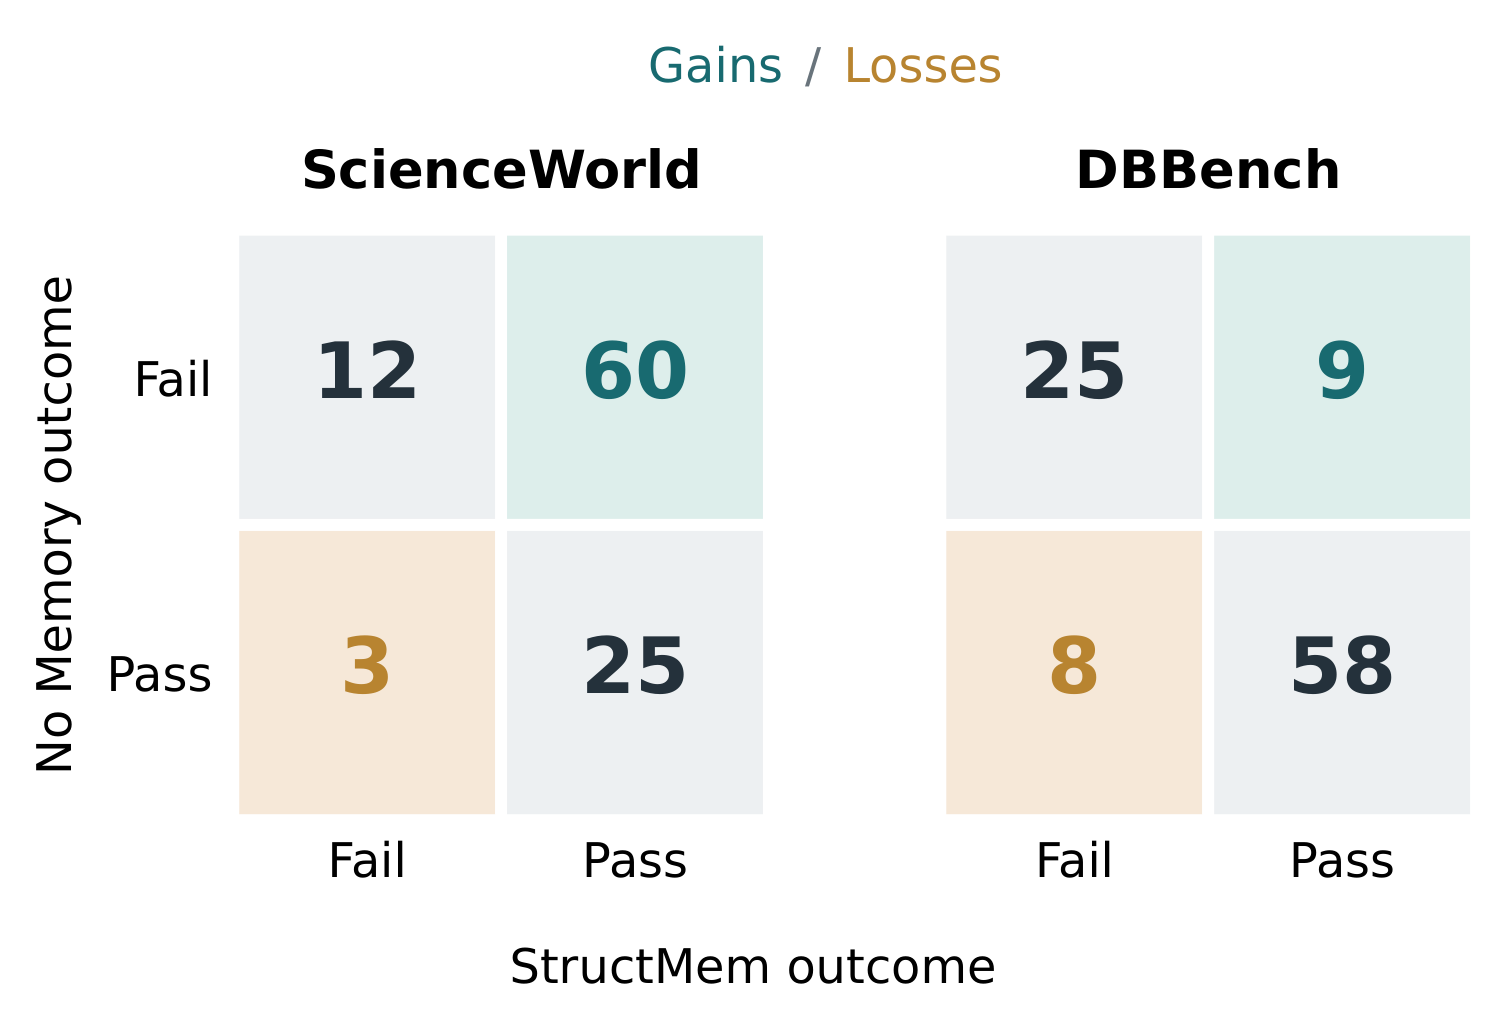
\includegraphics[width=\columnwidth]{figures/formal-paired.png}
  \caption{Paired terminal outcomes for No Memory (rows) and \SM{} (columns). Each panel counts the same 100 targets. Off-diagonal cells show gains and losses.}
  \Description{On ScienceWorld, 60 tasks pass only with StructMem and three pass only with No Memory. On DBBench, nine pass only with StructMem and eight only with No Memory.}
  \label{fig:paired}
\end{figure}

Figure~\ref{fig:paired} counts both directions of change. On ScienceWorld, 60 tasks succeed only with \SM{}, three only with No Memory, 25 with both, and 12 with neither. On DBBench, nine succeed only with \SM{}, eight only with No Memory, 58 with both, and 25 with neither. The DBBench total of one additional success therefore summarizes 17 disagreements. It provides little evidence that the integrated variant reliably improves read-query execution.

\begin{figure}[t]
  \centering
  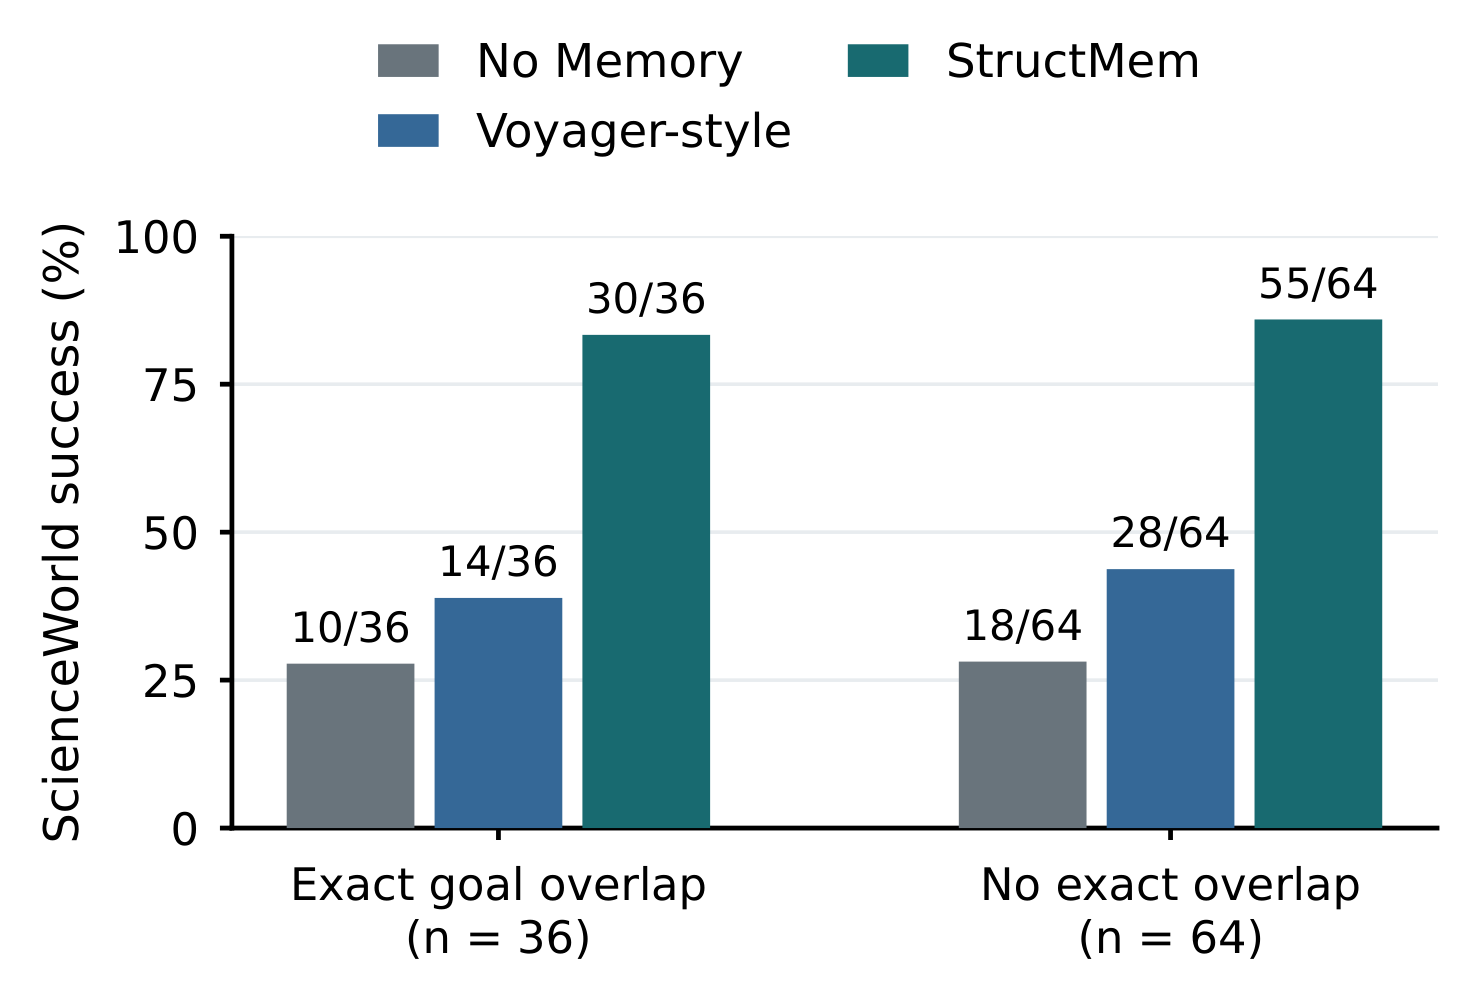
\includegraphics[width=\columnwidth]{figures/formal-overlap.png}
  \caption{ScienceWorld successes partitioned by exact normalized goal overlap with memory. Counts in each partition sum to the corresponding method's overall total.}
  \Description{Among 36 tasks with overlapping goals, No Memory, Voyager-style, and StructMem succeed on 10, 14, and 30. Among 64 without overlap, they succeed on 18, 28, and 55.}
  \label{fig:overlap}
\end{figure}

After excluding the 36 ScienceWorld targets with exact normalized source goal matches, \SM{} succeeds on 55 of 64 (85.9\%), Voyager-style on 28 (43.8\%), and No Memory on 18 (28.1\%). On the 36 overlapping targets the corresponding counts are 30, 14, and 10 (Figure~\ref{fig:overlap}). The full-system gap persists after removing exact matches. The partition can still contain common task templates and semantic near duplicates, and execution-specific logic remains part of the full agent.

The separate dense-only batch succeeds on 44 ScienceWorld and 62 DBBench targets out of 100. It also succeeds on 82 development-slice ALFWorld targets. That batch changes downstream processing and was collected separately. Measuring the independent effect of the structural channel would require comparing dense-plus-BM25 with the fused design under the same mapper, binder, executor, and inference allowance.

\subsection{Component removals and binding behavior}
\label{sec:removal}
\begin{figure}[t]
  \centering
  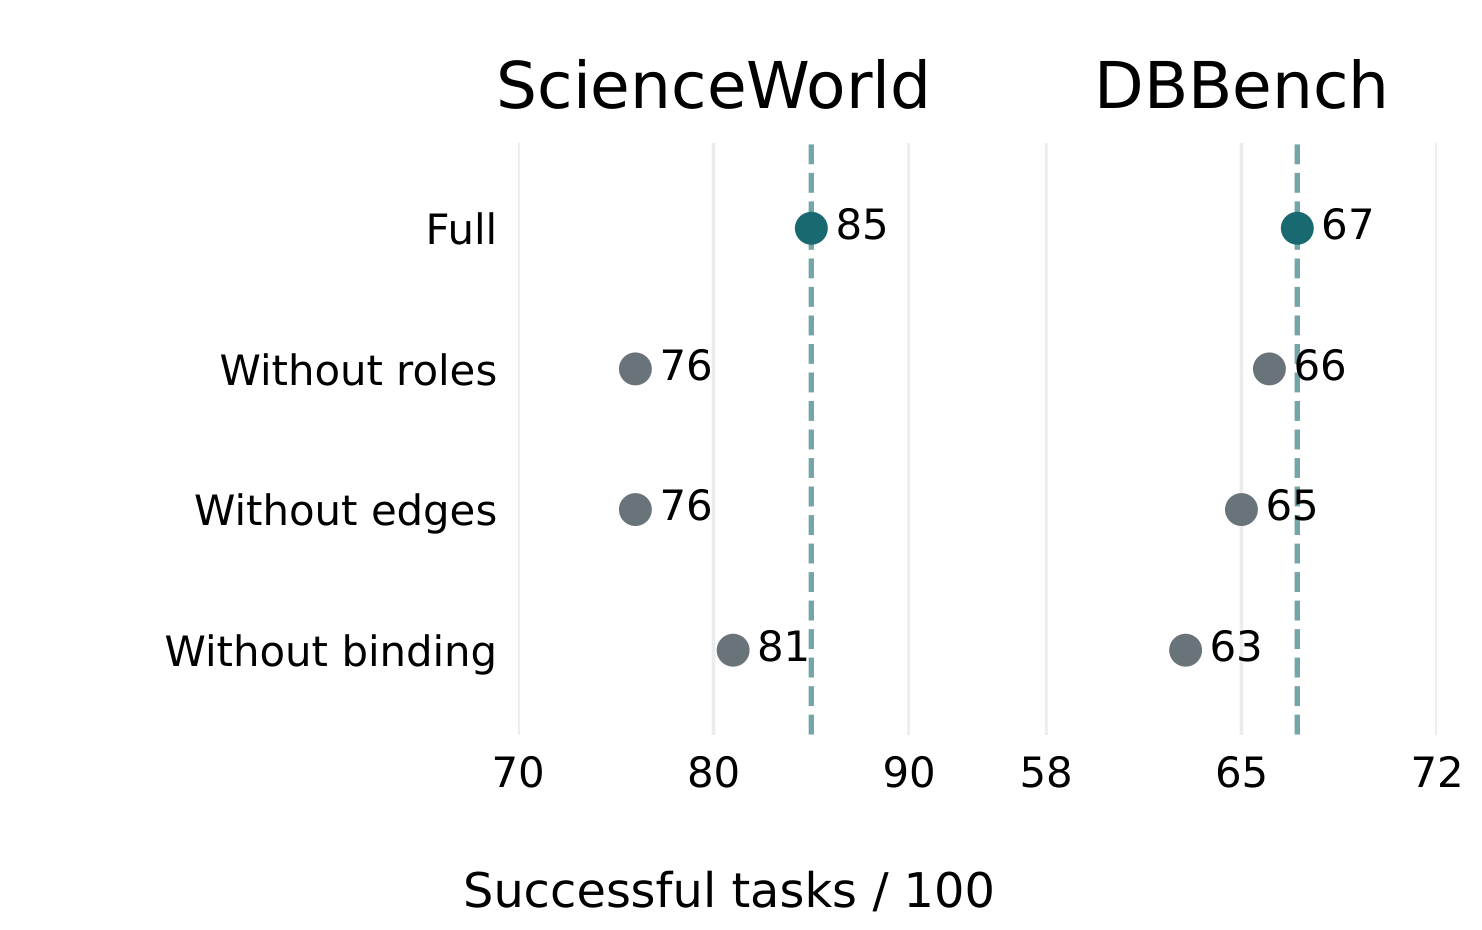
\includegraphics[width=\columnwidth]{figures/formal-removals.png}
  \caption{Single-component removals completed in the primary archive. Dashed lines mark the full integrated agent. The edge-feature removal retains graph density and length features.}
  \Description{Full, without roles, without edges, and without binding results are 85, 76, 76, and 81 on ScienceWorld and 67, 66, 65, and 63 on DBBench.}
  \label{fig:removals}
\end{figure}

Figure~\ref{fig:removals} retains the complete single-removal rows from the formal file. Removing roles or edge features reduces ScienceWorld successes from 85 to 76. Removing binding leaves 81. On DBBench the corresponding counts are 66, 65, and 63, compared with 67 for the full agent. Each removal changes inputs that downstream stages can use. The differences characterize the tested configurations and leave component interactions unresolved. The archived double and triple removals lack a common frozen version for factorial analysis.

\begin{figure}[t]
  \centering
  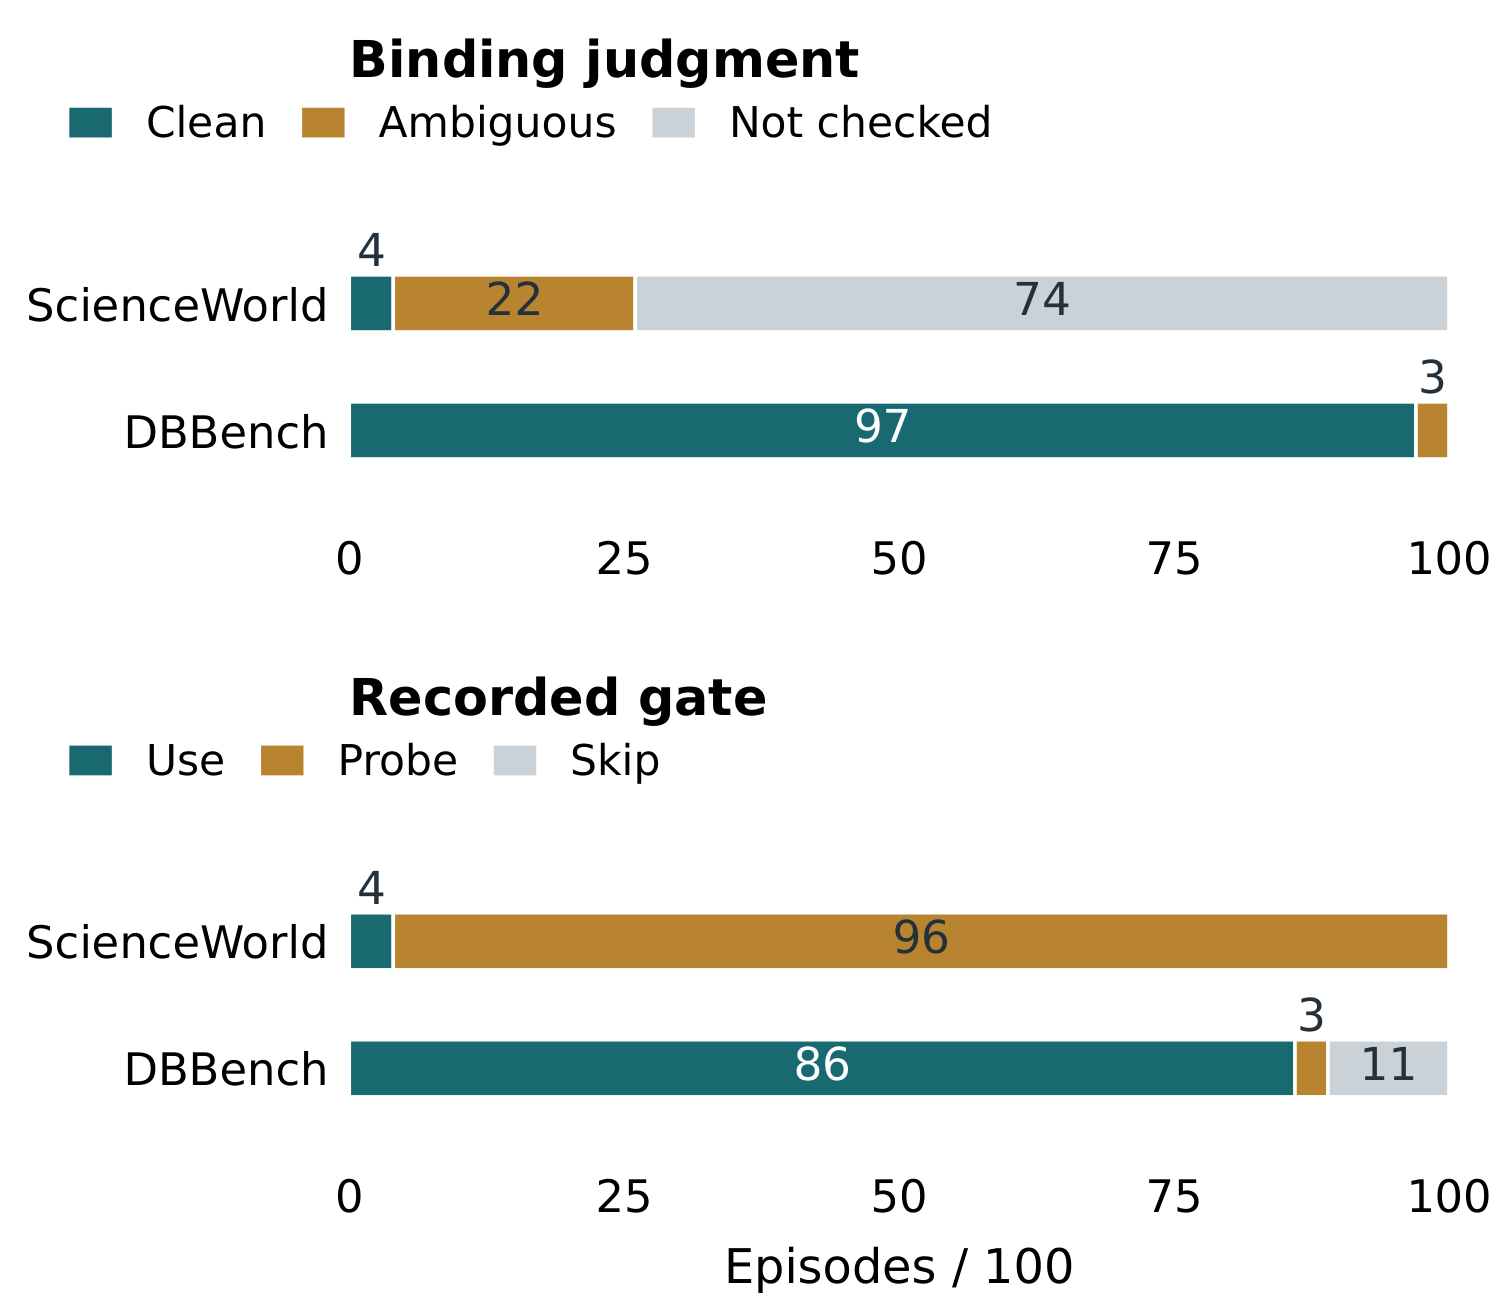
\includegraphics[width=\columnwidth]{figures/formal-binding.png}
  \caption{Binding judgments and gate states, each reported as a separate marginal distribution over 100 terminal episodes per workload. The counts describe logged judgments and control flow.}
  \Description{ScienceWorld binding records four clean, 22 ambiguous, and 74 not checked, with four use and 96 probe gate outcomes. DBBench records 97 clean and three ambiguous, with 86 use, three probe, and 11 skip.}
  \label{fig:binding}
\end{figure}

On ScienceWorld, the archive records 74 not-checked bindings, 22 ambiguous, and four clean. The gate records 96 probe and four use (Figure~\ref{fig:binding}). The number of not-checked episodes is consistent with execution paths bypassing the ordinary binder. The gate counts are a separate distribution, so the 96 probe states cannot be read as 96 completed binding checks or actions. On DBBench, 97 bindings are clean and three ambiguous, while the gate records 86 use, 11 skip, and three probe. The decrease from 97 clean judgments to 86 uses illustrates why the final control decision must be logged separately from the binding judgment.

These outputs describe the judgments and decisions that the agent recorded. Independent relevance or applicability assessment would require labeling procedures, bindings, and feedback external to the system. The archive's analogous-reference IDs and score-defined bins are derived from the same retrieval mechanism. Evaluating ranking quality on them would reward agreement with the proxy rather than skill at finding reusable procedures.

\subsection{SQL query strata and endpoint sensitivity}
\label{sec:sql}
\begin{table}[t]
  \caption{Primary DBBench successes by declared query type. Aggregation pools SUM, MIN, MAX, and AVG. Each target is a read query.}
  \label{tab:strata}
  \begin{tabular*}{\columnwidth}{@{\extracolsep{\fill}}lrrr@{}}
    \toprule
    Query type & Tasks & No Memory & \SM{} \\
    \midrule
    Lookup / other & 17 & 15 & 12 \\
    Counting       & 17 & 9  & 9  \\
    Comparison     & 17 & 10 & 13 \\
    Ranking        & 17 & 9  & 10 \\
    Aggregation    & 32 & 23 & 23 \\
    \midrule
    Total          & 100 & 66 & 67 \\
    \bottomrule
  \end{tabular*}
\end{table}

Table~\ref{tab:strata} groups queries by existing workload labels. Relative to No Memory, \SM{} gains three comparison successes and one ranking success, loses three lookup/other successes, and ties on counting and aggregation. The overall difference pools positive, negative, and zero changes. Small strata and one terminal result per target limit interpretation of the type-level differences.

On the secondary DBBench endpoint, \SM{} succeeds on 58 tasks and No Memory on 65. Reflexion-style and MemGPT-style each succeed on 68. The reverse ordering of \SM{} and No Memory relative to the primary endpoint makes the result endpoint-dependent in these batches. Retrieval changes which procedures are supplied, while rendering those procedures as executable actions and answer formats still depends on the model and execution rules. The endpoint comparison leaves the source of the reversal unresolved.

\subsection{Recorded inference and screening cost}
\label{sec:cost}
\begin{table}[t]
  \caption{Primary archive means over 100 terminal tasks per configuration. Tokens are recorded input plus output usage, including cached-response usage. Decisions count environment-facing agent steps.}
  \label{tab:usage}
  \begin{tabular*}{\columnwidth}{@{\extracolsep{\fill}}llrr@{}}
    \toprule
    Workload & Agent & Tokens (k) & Decisions \\
    \midrule
    ScienceWorld & No Memory     & 27.7 & 37.9 \\
                 & Voyager-style & 76.0 & 33.9 \\
                 & \SM{}         & 15.2 & 16.9 \\
    \addlinespace
    DBBench      & No Memory     & 1.5  & 2.5  \\
                 & Voyager-style & 6.7  & 2.3  \\
                 & \SM{}         & 14.3 & 2.1  \\
    \bottomrule
  \end{tabular*}
\end{table}

\begin{figure*}[t]
  \centering
  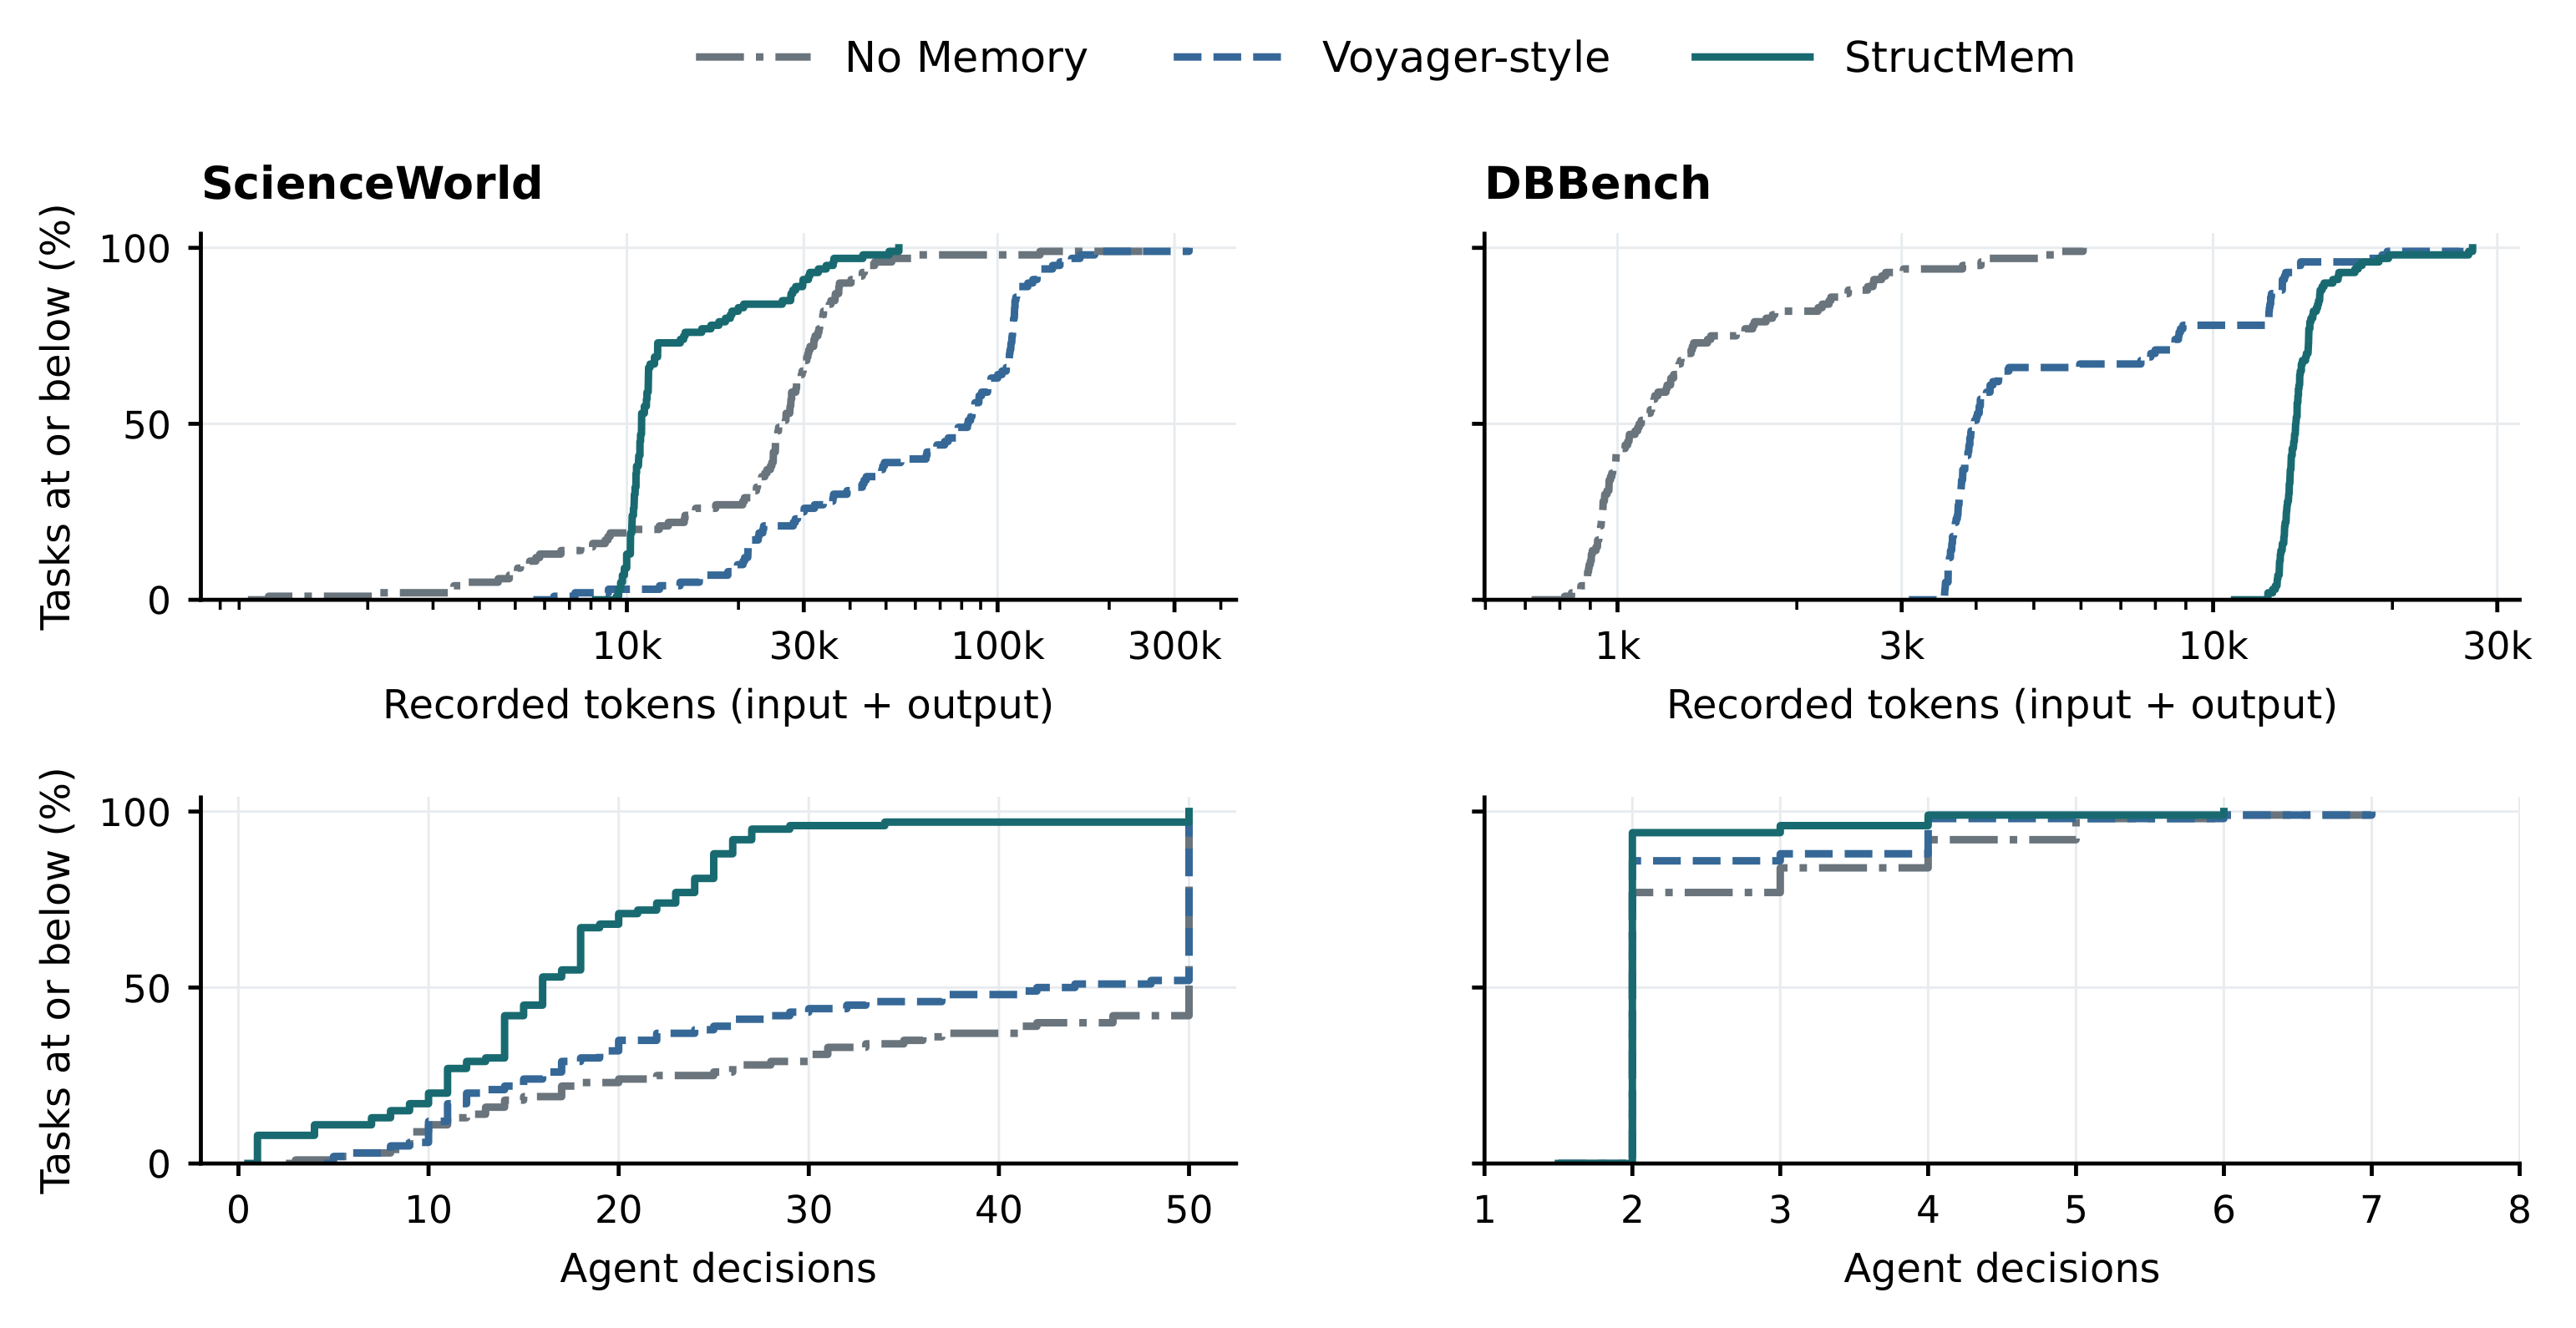
\includegraphics[width=\textwidth]{figures/formal-usage.png}
  \caption{Empirical cumulative distributions of recorded tokens (top, log-scaled) and decisions (bottom). Each curve includes all 100 terminal tasks, including failures.}
  \Description{Four panels compare No Memory, Voyager-style, and StructMem across ScienceWorld and DBBench. StructMem uses fewer decisions and tokens on ScienceWorld, and more tokens on DBBench.}
  \label{fig:usage}
\end{figure*}

Table~\ref{tab:usage} reports means for three configurations. On ScienceWorld, \SM{} records fewer tokens and decisions than No Memory. This is consistent with the specialized routines in Section~\ref{sec:execution}. On DBBench, \SM{} records 14.3k tokens per task compared with 1.5k for No Memory, with a single additional success. The added representation, adaptation, and binding work can be large relative to a short SQL interaction. The recorded means exclude failed agent attempts and do not estimate how much retrying costs.

The distributions in Figure~\ref{fig:usage} expose differences hidden by the means. In ScienceWorld, \SM{}, No Memory, and Voyager-style record median usages of 11.0k, 26.7k, and 83.1k tokens. The respective counts at the 50-decision limit are 3, 58, and 48. The DBBench median is two decisions for all three configurations, while median token usage is 13.8k for \SM{} and 1.1k for No Memory. Model-side and environment-facing work therefore respond differently to the added pipeline. Cached usage and omitted retry work prevent a corresponding comparison of billed cost or live latency.

\begin{figure}[t]
  \centering
  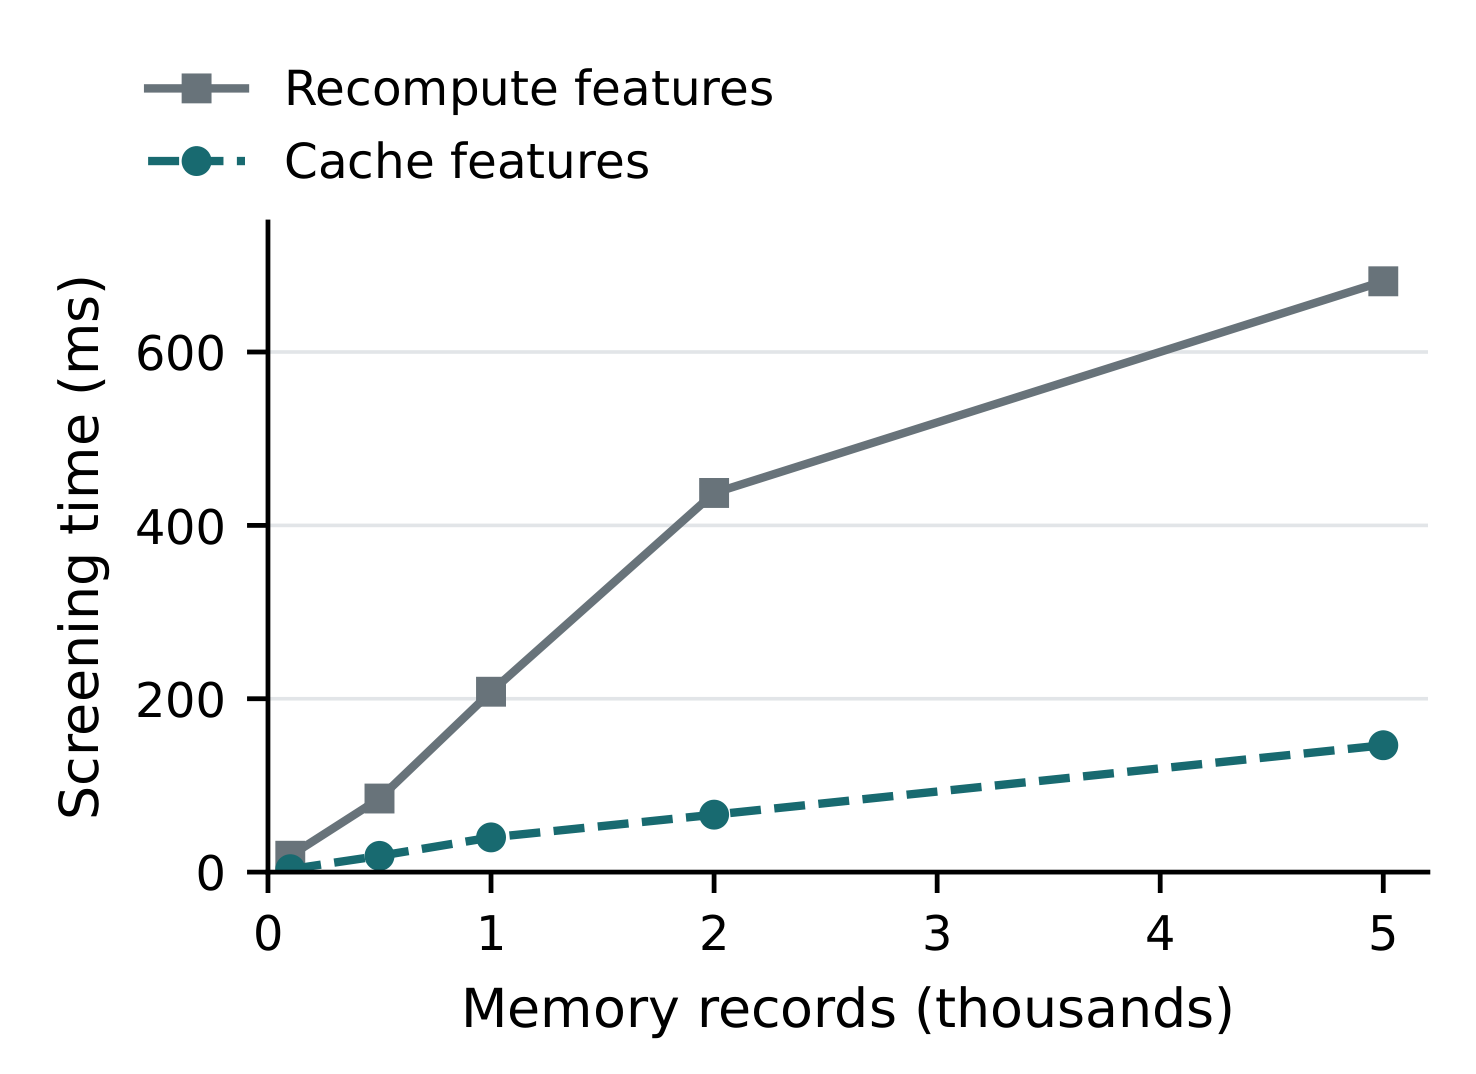
\includegraphics[width=\columnwidth]{figures/formal-screening.png}
  \caption{Saved structural screening microbenchmark on synthetic eight-action records. Each point sums saved component minima. The cached variant excludes source feature preparation.}
  \Description{A curve for recomputed source features rises faster than the cached-feature curve over the measured range of 100 to 5,000 records.}
  \label{fig:screening}
\end{figure}

Figure~\ref{fig:screening} uses saved component timings for 100 to 5,000 synthetic eight-action records. At 1,000 records, component minima sum to 208.1 ms with feature recomputation and 40.1 ms with cached features. The cached variant avoids repeated source feature extraction while retaining sequence comparison and sorting. The saved record omits hardware details and reports minima. These timings characterize the recorded structural pass. Dense and lexical ranking, model calls, and environment interaction have their own latency and fall outside the measurement.
